\chapter{Architettura del Calcolatore}

L'architettura del calcolatore descrive \emph{come è fatta e come funziona} una CPU con la sua memoria: quali unità la compongono, come eseguono le istruzioni, come la \textbf{pipeline} ne aumenta la velocità e come la \textbf{gerarchia di memoria} nasconde la lentezza della RAM. Nella Sezione A è uscita come tema di Elettronica (prima sessione 2024: datapath RISC e pipeline; prima sessione 2018: struttura interna di un microcontrollore). Il capitolo termina con la risposta svolta al tema 2024.

Gli esempi usano \textbf{RISC-V} (architettura RISC aperta, la più semplice da studiare); i concetti valgono anche per MIPS e ARM. I numeri dei diagrammi di pipeline sono stati verificati con un piccolo simulatore.

\section{Il Modello di von Neumann}

\subsection{Componenti}
\begin{itemize}
    \item \textbf{CPU}: \textbf{unità di controllo} (decodifica le istruzioni e genera i segnali di controllo), \textbf{ALU} (operazioni aritmetiche e logiche), \textbf{registri} (memoria velocissima dentro la CPU), tra cui il \textbf{Program Counter} (PC, indirizzo della prossima istruzione) e il registro delle istruzioni.
    \item \textbf{Memoria}: contiene \emph{sia le istruzioni sia i dati} (``programma memorizzato'', \emph{stored program}).
    \item \textbf{Ingresso/uscita} (I/O): periferiche, collegate tramite controller.
    \item \textbf{Bus}: collegamenti condivisi (indirizzi, dati, controllo).
\end{itemize}

\subsection{Il ciclo di istruzione}
La CPU ripete all'infinito: \textbf{fetch} (legge l'istruzione all'indirizzo del PC), \textbf{decode} (decodifica e legge i registri), \textbf{execute} (calcola), \textbf{memory} (accede ai dati, se serve), \textbf{write back} (scrive il risultato) e aggiorna il PC (di norma $\text{PC}\leftarrow\text{PC}+4$; un salto lo sostituisce con l'indirizzo di destinazione).

\subsection{Perché ``programma memorizzato''}
Se il programma è in memoria come i dati, cambiare programma significa solo caricarne un altro: lo stesso hardware esegue qualunque software (un compilatore produce dati che sono programmi). È la base di ogni calcolatore moderno.

\subsection{Von Neumann e Harvard}
\begin{itemize}
    \item \textbf{Von Neumann}: una sola memoria e un solo bus per istruzioni e dati $\Rightarrow$ il \textbf{collo di bottiglia di von Neumann}: CPU veloce e memoria lenta, e non si può leggere un'istruzione e un dato nello stesso ciclo.
    \item \textbf{Harvard}: memorie e bus \textbf{separati} per istruzioni e dati: si accede a entrambe nello stesso ciclo. È la scelta tipica dei \textbf{microcontrollori} e, \emph{dentro la CPU}, delle cache di primo livello (cache istruzioni e cache dati separate): le CPU moderne sono ``von Neumann'' verso la RAM e ``Harvard'' verso la cache.
\end{itemize}

\section{Richiami di Reti Logiche}
Il datapath e la pipeline sono costruiti con due tipi di circuiti digitali.
\begin{itemize}
    \item \textbf{Reti combinatorie}: l'uscita dipende \emph{solo} dagli ingressi attuali (porte logiche, \textbf{multiplexer} che sceglie un ingresso, \textbf{decoder}, \textbf{addizionatore}, \textbf{ALU}). Hanno un ritardo di propagazione.
    \item \textbf{Reti sequenziali}: l'uscita dipende anche dallo \textbf{stato}, memorizzato in \textbf{flip-flop} e \textbf{registri} aggiornati sul fronte del \textbf{clock}. Un \textbf{registro} memorizza una parola; un \textbf{register file} ne raccoglie molti con porte di lettura e scrittura. Una \textbf{macchina a stati finiti} (FSM) è la base dell'unità di controllo.
    \item \textbf{Perché il clock}: sincronizza il sistema. Il periodo del clock deve essere \textbf{maggiore del cammino combinatorio più lungo} tra due registri (più i tempi di setup), altrimenti il dato non fa in tempo ad arrivare. La frequenza è l'inverso del periodo.
    \item \textbf{Sommatore}: il \emph{ripple-carry} propaga il riporto bit a bit (ritardo proporzionale al numero di bit); il \emph{carry-lookahead} calcola i riporti in parallelo, più veloce e più costoso.
\end{itemize}

\section{Instruction Set Architecture (ISA)}
L'\textbf{ISA} è il \emph{contratto} tra software e hardware: insieme delle istruzioni, registri, modi di indirizzamento, formato in memoria. Il compilatore produce istruzioni per un'ISA; molte implementazioni hardware diverse la realizzano (stessa ISA, microarchitetture diverse).

\subsection{RISC e CISC}
\begin{center}
\small
\begin{tabularx}{\textwidth}{@{}>{\raggedright\arraybackslash}p{3.1cm}XX@{}}
\toprule
 & \textbf{RISC} (RISC-V, MIPS, ARM) & \textbf{CISC} (x86) \\
\midrule
Istruzioni & Poche, semplici, tutte della \textbf{stessa lunghezza} (32 bit) & Molte, complesse, \textbf{lunghezza variabile} \\
Accesso alla memoria & \textbf{Load/store}: solo \texttt{lw} e \texttt{sw} accedono alla memoria; le altre operano sui registri & Molte istruzioni operano direttamente su operandi in memoria \\
Registri & Molti (32) & Meno (storicamente) \\
Decodifica & Semplice e veloce & Complessa (spesso tradotta in micro-operazioni RISC-like) \\
Vantaggio & Hardware semplice, \textbf{pipeline efficiente}, bassa potenza & Codice più compatto, compatibilità storica \\
Esempi & Smartphone, microcontrollori, server (ARM), RISC-V & PC e server x86 \\
\bottomrule
\end{tabularx}
\end{center}
\textbf{Perché RISC}: istruzioni uniformi e semplici rendono facile dividere l'esecuzione in stadi di uguale durata, cioè fare la pipeline (vedi più avanti). Oggi la differenza si è attenuata: i processori x86 traducono internamente le istruzioni in micro-operazioni simili a quelle RISC.

\subsection{RISC-V: registri e formati}
\begin{itemize}
    \item \textbf{32 registri} a 32 bit (\texttt{x0}\ldots\texttt{x31}); \texttt{x0} vale \textbf{sempre zero}. Convenzioni: \texttt{sp} (stack pointer), \texttt{ra} (indirizzo di ritorno), \texttt{a0}--\texttt{a7} (argomenti e valore di ritorno), \texttt{t0}--\texttt{t6} (temporanei), \texttt{s0}--\texttt{s11} (da preservare). Le chiamate di funzione usano lo stack con il record di attivazione (vedi i capitoli \emph{Sistemi Operativi} e \emph{Programmazione}).
    \item \textbf{Formato R} (registro--registro): \texttt{funct7 | rs2 | rs1 | funct3 | rd | opcode}. Esempio \texttt{add x1, x2, x3}.
    \item \textbf{Formato I} (immediato, \texttt{lw}): \texttt{imm[11:0] | rs1 | funct3 | rd | opcode}. \textbf{Formato S} (\texttt{sw}): immediato diviso in due parti. \textbf{Formato B} (salti condizionati): offset di salto.
\end{itemize}
Esempi di codifica a 32 bit (verificati):
\begin{center}
\small
\begin{tabular}{@{}llc@{}}
\toprule
\textbf{Istruzione} & \textbf{Significato} & \textbf{Codice (esadecimale)} \\
\midrule
\texttt{add x1, x2, x3} & $x_1 \leftarrow x_2 + x_3$ & \texttt{003100B3} \\
\texttt{sub x5, x6, x7} & $x_5 \leftarrow x_6 - x_7$ & \texttt{407302B3} \\
\texttt{addi x5, x0, 10} & $x_5 \leftarrow 10$ & \texttt{00A00293} \\
\texttt{lw x6, 8(x7)} & $x_6 \leftarrow \text{Mem}[x_7 + 8]$ & \texttt{0083A303} \\
\texttt{sw x6, 8(x7)} & $\text{Mem}[x_7 + 8] \leftarrow x_6$ & \texttt{0063A423} \\
\texttt{beq x1, x2, +16} & se $x_1 = x_2$: $\text{PC} \leftarrow \text{PC} + 16$ & \texttt{00208863} \\
\bottomrule
\end{tabular}
\end{center}

\subsection{Modi di indirizzamento}
\textbf{Registro} (operandi nei registri), \textbf{immediato} (costante nell'istruzione), \textbf{base + spostamento} (\texttt{lw x6, 8(x7)}), \textbf{relativo al PC} (salti), \textbf{pseudo-diretto} (jump). \textbf{Perché pochi}: ogni modo complica decodifica e pipeline.

\subsection{Esempio: da C ad assembly}
Somma degli elementi di un vettore di 4 interi (\texttt{x10} = indirizzo base).
\begin{lstlisting}[numbers=none, caption={Somma di un vettore in assembly RISC-V (eseguita su un simulatore)}]
        addi x5, x0, 0        # somma = 0
        addi x6, x0, 0        # i = 0
        addi x7, x0, 4        # n = 4
loop:   slli x8, x6, 2        # offset = i * 4  (ogni intero e' 4 byte)
        add  x8, x8, x10      # indirizzo di a[i]
        lw   x9, 0(x8)        # x9 = a[i]
        add  x5, x5, x9       # somma += a[i]
        addi x6, x6, 1        # i++
        bne  x6, x7, loop     # se i != n, ripeti
\end{lstlisting}
Con $a = [1,2,3,4]$ il programma esegue \textbf{27 istruzioni} (3 di inizializzazione e 4 iterazioni da 6) e lascia $x_5 = 10$.

\section{Il Datapath}
Il \textbf{datapath} è l'insieme di unità funzionali e collegamenti che eseguono le istruzioni; l'\textbf{unità di controllo} stabilisce, per ogni istruzione, quali unità si usano e come.

\subsection{Unità funzionali}
\begin{center}
\small
\begin{tabularx}{\textwidth}{@{}>{\raggedright\arraybackslash}p{3.4cm}X@{}}
\toprule
\textbf{Unità} & \textbf{Funzione} \\
\midrule
\textbf{Program Counter (PC)} & Registro con l'indirizzo dell'istruzione da eseguire \\
\textbf{Sommatore PC + 4} & Calcola l'indirizzo dell'istruzione successiva (le istruzioni sono lunghe 4 byte) \\
\textbf{Memoria istruzioni} & Dato l'indirizzo (PC), restituisce l'istruzione (di sola lettura) \\
\textbf{Register file} & Banco di registri con \textbf{due porte di lettura} (\texttt{rs1}, \texttt{rs2}) e \textbf{una di scrittura} (\texttt{rd}, abilitata da \texttt{RegWrite}) \\
\textbf{Generatore di immediati} & Estende con il segno la costante contenuta nell'istruzione \\
\textbf{ALU} & Esegue somma, sottrazione, AND, OR, confronti; calcola anche l'\emph{indirizzo} di \texttt{lw}/\texttt{sw} (registro base + spostamento) e confronta nei salti condizionati \\
\textbf{Memoria dati} & Lettura (\texttt{lw}) e scrittura (\texttt{sw}) dei dati \\
\textbf{Sommatore dei salti} & Calcola l'indirizzo di destinazione $\text{PC} + \text{offset}$ \\
\textbf{Multiplexer} & Scelgono tra più sorgenti (secondo operando dell'ALU: registro o immediato; dato da scrivere nel registro: ALU o memoria; prossimo PC: $\text{PC}+4$ o destinazione del salto) \\
\textbf{Unità di controllo} & Legge l'\emph{opcode} e genera i segnali di controllo \\
\bottomrule
\end{tabularx}
\end{center}

\subsection{Segnali di controllo}
\begin{center}
\small
\begin{tabularx}{\textwidth}{@{}>{\raggedright\arraybackslash}p{2.2cm}cccccc@{}}
\toprule
\textbf{Istruzione} & \textbf{RegWrite} & \textbf{ALUSrc} & \textbf{MemRead} & \textbf{MemWrite} & \textbf{MemtoReg} & \textbf{Branch} \\
\midrule
Tipo R (\texttt{add}) & 1 & registro & 0 & 0 & ALU & 0 \\
\texttt{lw} & 1 & immediato & 1 & 0 & memoria & 0 \\
\texttt{sw} & 0 & immediato & 0 & 1 & -- & 0 \\
\texttt{beq} & 0 & registro & 0 & 0 & -- & 1 \\
\bottomrule
\end{tabularx}
\end{center}

\subsection{Quali unità usa ciascuna istruzione}
\begin{itemize}
    \item \textbf{Tipo R} (\texttt{add x1,x2,x3}): memoria istruzioni $\to$ register file (legge $x_2$, $x_3$) $\to$ ALU (somma) $\to$ register file (scrive $x_1$). \emph{Non usa la memoria dati.}
    \item \textbf{\texttt{lw}}: legge $x_{\text{base}}$ $\to$ ALU (base $+$ spostamento) $\to$ \textbf{memoria dati} (lettura) $\to$ scrive il registro destinazione.
    \item \textbf{\texttt{sw}}: legge base e dato $\to$ ALU (indirizzo) $\to$ \textbf{memoria dati} (scrittura). \emph{Non scrive nei registri.}
    \item \textbf{\texttt{beq}}: legge due registri $\to$ ALU (confronto) $\to$ se uguali, il sommatore dei salti sostituisce il PC.
\end{itemize}

\subsection{Datapath a ciclo singolo e perché non basta}
Nel datapath \textbf{a ciclo singolo} ogni istruzione si esegue in \emph{un solo ciclo di clock}. Il periodo deve però bastare per l'istruzione \emph{più lenta} (\texttt{lw}, che usa tutte le unità): con ritardi tipici (accesso a memoria istruzioni 200 ps, lettura registri 100 ps, ALU 200 ps, memoria dati 200 ps, scrittura registri 100 ps) il periodo è di $800$ ps, anche per istruzioni che sarebbero state più rapide. Inoltre ogni unità è usata solo in una piccola frazione del ciclo: \textbf{si spreca hardware}. La \textbf{pipeline} risolve entrambi i problemi.

\section{La Pipeline}

\subsection{L'idea}
Si divide l'esecuzione in \textbf{stadi} e, \emph{mentre un'istruzione è in un certo stadio, la successiva occupa lo stadio precedente}: come in una catena di montaggio (o una lavanderia con lavatrice, asciugatrice e stiro che lavorano insieme su carichi diversi). Ogni unità lavora \emph{in ogni ciclo}, su un'istruzione diversa.

\subsection{I cinque stadi (RISC classico)}
\begin{center}
\small
\begin{tabularx}{\textwidth}{@{}>{\raggedright\arraybackslash}p{2.4cm}XX@{}}
\toprule
\textbf{Stadio} & \textbf{Che cosa avviene} & \textbf{Unità funzionali coinvolte} \\
\midrule
\textbf{IF} -- \emph{Instruction Fetch} & Si legge l'istruzione all'indirizzo del PC e si calcola $\text{PC}+4$ & PC, memoria istruzioni, sommatore $+4$ \\
\textbf{ID} -- \emph{Instruction Decode} & Si decodifica l'istruzione, si leggono i registri sorgente, si estende l'immediato, si generano i segnali di controllo & Unità di controllo, \textbf{register file} (lettura), generatore di immediati, unità di rilevamento degli hazard \\
\textbf{EX} -- \emph{Execute} & Si esegue l'operazione, si calcola l'indirizzo di memoria o di salto, si confrontano i registri & \textbf{ALU}, sommatore dei salti, multiplexer degli operandi, unità di forwarding \\
\textbf{MEM} -- \emph{Memory} & Si legge o si scrive la memoria dati (solo \texttt{lw}/\texttt{sw}); nei salti si decide il PC & \textbf{Memoria dati} \\
\textbf{WB} -- \emph{Write Back} & Si scrive il risultato (ALU o memoria) nel registro destinazione & \textbf{Register file} (scrittura), multiplexer \\
\bottomrule
\end{tabularx}
\end{center}

\begin{figure}[h!]
    \centering
    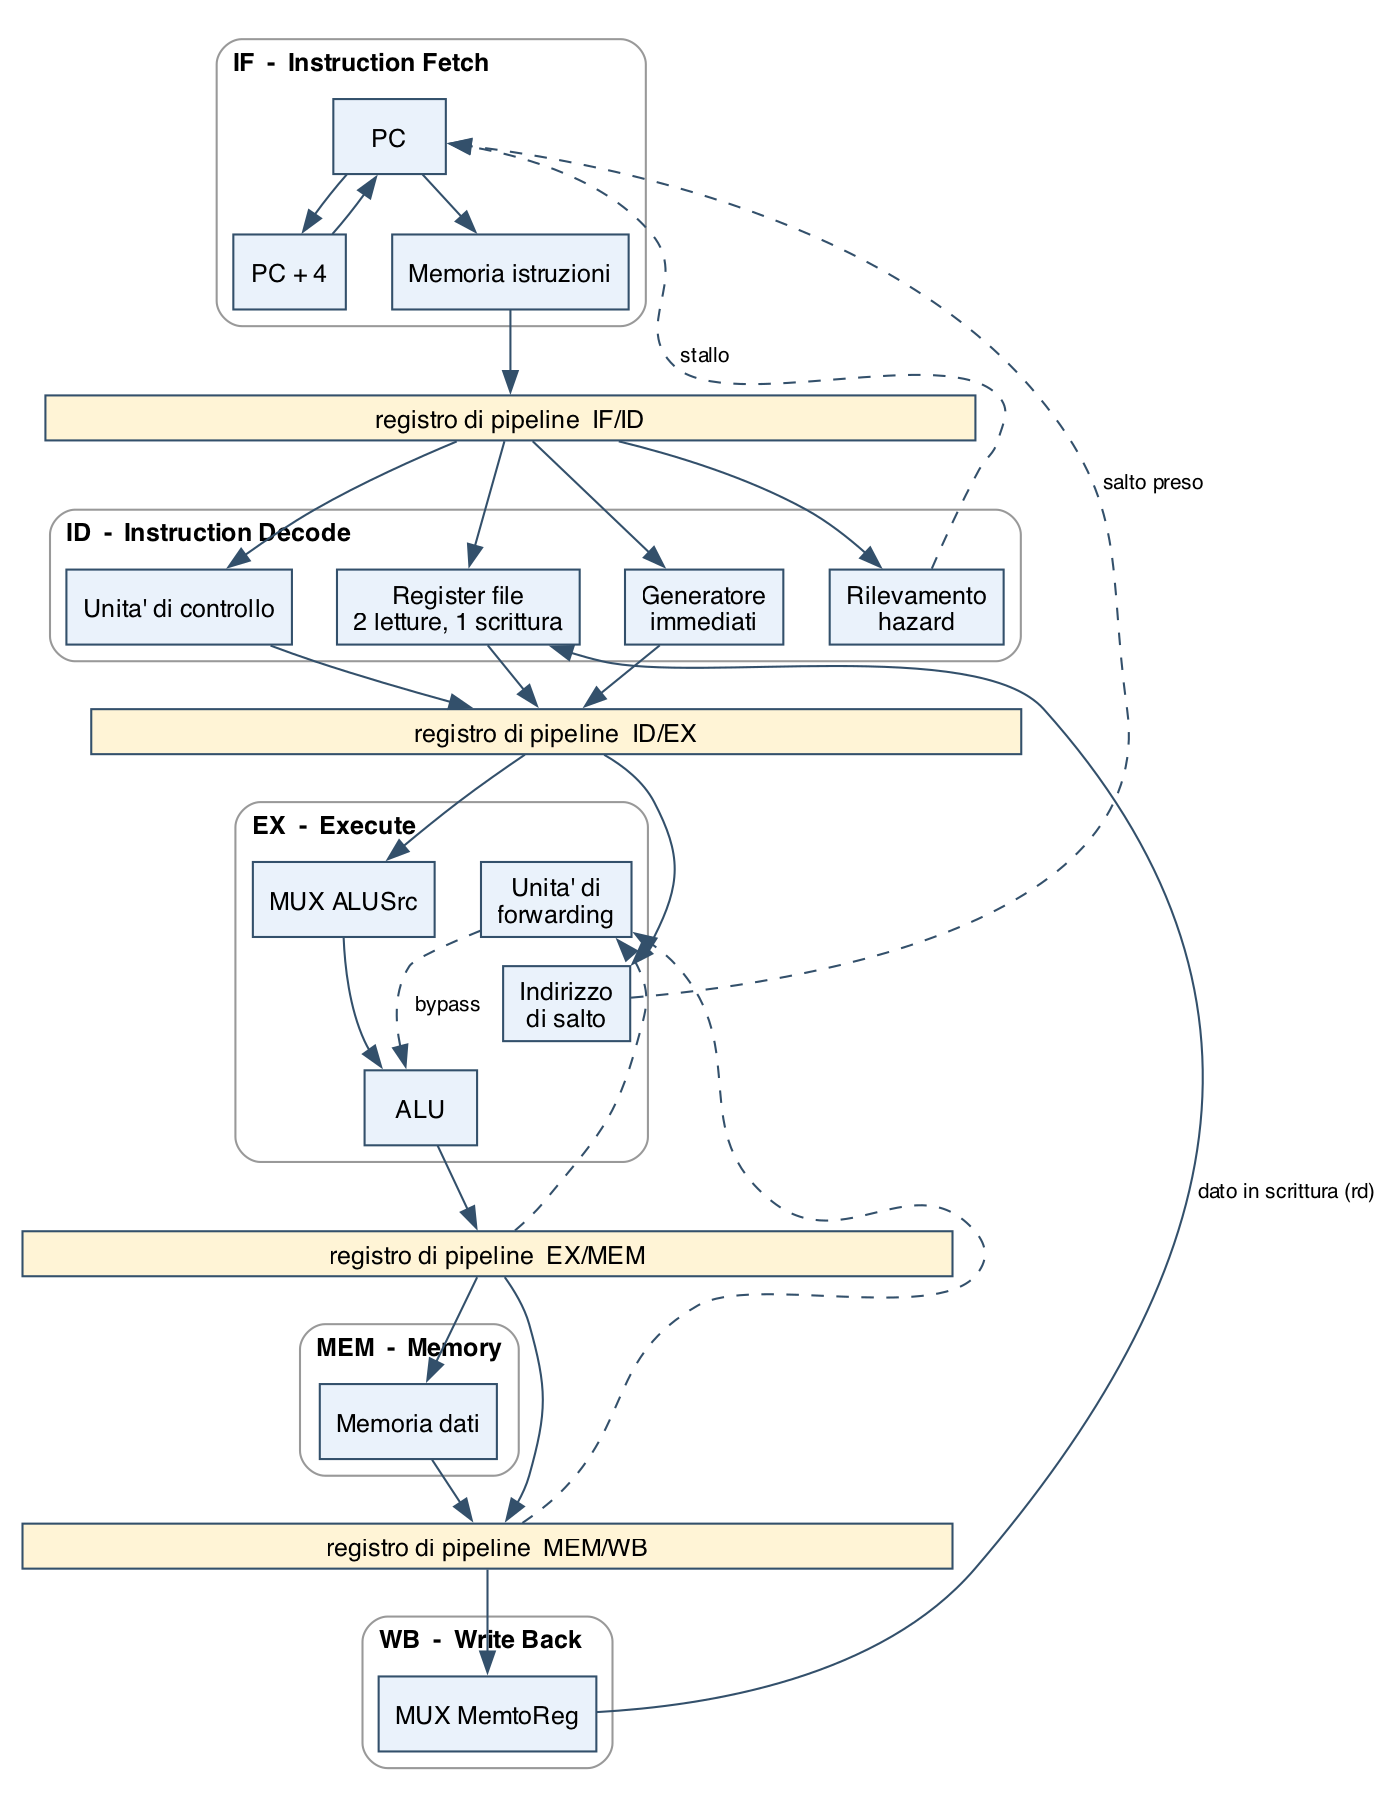
\includegraphics[width=0.78\textwidth]{immagini/pipeline_5_stadi_riscv.png}
    \caption{Datapath a pipeline a cinque stadi: i registri di pipeline separano gli stadi; le linee tratteggiate sono l'unità di forwarding, il rilevamento degli hazard e il salto preso.}
    \label{fig:pipeline}
\end{figure}

\subsection{Registri di pipeline}
Tra gli stadi si inseriscono \textbf{registri di pipeline} (\texttt{IF/ID}, \texttt{ID/EX}, \texttt{EX/MEM}, \texttt{MEM/WB}). \textbf{Perché}: a ogni ciclo ogni stadio lavora su un'istruzione diversa, quindi i dati e i segnali di controllo di ciascuna istruzione devono essere \emph{conservati} mentre procede da uno stadio al successivo; senza registri, il risultato di un'istruzione sarebbe sovrascritto da quella che la segue.

\subsection{Diagramma temporale}
Cinque istruzioni indipendenti (una colonna per ciclo di clock):
\begin{center}
\small
\begin{tabular}{@{}l|ccccccccc@{}}
 & 1 & 2 & 3 & 4 & 5 & 6 & 7 & 8 & 9 \\
\hline
istruzione 1 & IF & ID & EX & MEM & WB & & & & \\
istruzione 2 & & IF & ID & EX & MEM & WB & & & \\
istruzione 3 & & & IF & ID & EX & MEM & WB & & \\
istruzione 4 & & & & IF & ID & EX & MEM & WB & \\
istruzione 5 & & & & & IF & ID & EX & MEM & WB \\
\end{tabular}
\end{center}
Dal ciclo 5 la pipeline è \emph{piena}: ogni ciclo termina un'istruzione. Con $k$ stadi, $n$ istruzioni richiedono $k + (n-1)$ cicli.

\subsection{Vantaggi, con i numeri}
Con gli stessi ritardi di prima (200, 100, 200, 200, 100 ps):
\begin{itemize}
    \item \textbf{Ciclo singolo}: periodo $= 800$ ps; $1000$ istruzioni $\Rightarrow 1000\cdot 800 = 800\,000$ ps.
    \item \textbf{Pipeline}: il periodo è il ritardo dello stadio \emph{più lento}, $200$ ps; $1000$ istruzioni $\Rightarrow (1000+4)\cdot 200 = 200\,800$ ps.
    \item \textbf{Accelerazione} $= 800\,000/200\,800 \approx \mathbf{3{,}98}$ (non 5: gli stadi non sono bilanciati; con stadi uguali l'accelerazione ideale tende al numero di stadi).
    \item \textbf{Throughput} (istruzioni al secondo): aumenta, idealmente a una istruzione per ciclo ($\text{CPI}\to 1$) con un clock più veloce.
    \item \textbf{Latenza} di una singola istruzione: \emph{non migliora}, anzi peggiora: $5\cdot 200 = 1000$ ps contro $800$ ps. La pipeline migliora il \emph{numero di istruzioni completate per unità di tempo}, non il tempo di una singola.
    \item \textbf{Utilizzo dell'hardware}: ogni unità lavora ad ogni ciclo.
\end{itemize}

\section{Hazard: i Problemi della Pipeline}
Un \textbf{hazard} è una situazione in cui l'istruzione successiva \emph{non può} entrare nel ciclo seguente. Se non gestito, produce risultati sbagliati o richiede di fermare (\emph{stallo}) la pipeline.

\subsection{Hazard strutturali}
Due istruzioni vogliono usare la \emph{stessa risorsa} nello stesso ciclo. Esempio: con \emph{una sola memoria} per istruzioni e dati, \texttt{lw} nello stadio MEM e il fetch di un'istruzione successiva nello stadio IF vorrebbero la memoria insieme. \textbf{Soluzione}: duplicare la risorsa (memoria istruzioni e memoria dati separate, o cache separate: architettura Harvard); register file con scrittura nella prima metà del ciclo e lettura nella seconda.

\subsection{Hazard sui dati}
Un'istruzione usa un risultato di una precedente \emph{non ancora scritto} nel registro (dipendenza \textbf{RAW}, \emph{read after write}):
\begin{lstlisting}[numbers=none, caption={Dipendenza RAW}]
add x1, x2, x3     # scrive x1 nello stadio WB (ciclo 5)
sub x4, x1, x5     # legge x1 nello stadio ID (ciclo 3): valore ANCORA VECCHIO
\end{lstlisting}
\textbf{Soluzioni}
\begin{itemize}
    \item \textbf{Stallo} (\emph{bolla}): si inseriscono cicli vuoti finché il dato è pronto. Senza altre misure sono \textbf{2 cicli} se l'istruzione dipendente segue subito, \textbf{1 ciclo} se c'è un'istruzione nel mezzo.
    \item \textbf{Forwarding} (\emph{bypass}): il risultato dell'ALU è \emph{inoltrato} direttamente dai registri \texttt{EX/MEM} o \texttt{MEM/WB} all'ingresso dell'ALU, senza aspettare la scrittura nel register file. \textbf{Perché funziona}: il dato è già calcolato alla fine dello stadio EX, solo non ancora ``ufficialmente'' scritto. Un multiplexer in ingresso all'ALU e un'\textbf{unità di forwarding} che confronta i numeri di registro lo realizzano. Elimina quasi tutti gli stalli sulle istruzioni aritmetiche.
    \item \textbf{Il caso \emph{load-use}}: dopo un \texttt{lw} il dato è disponibile solo alla fine dello stadio \textbf{MEM}, troppo tardi per essere usato nello stadio EX dell'istruzione successiva: anche con il forwarding serve \textbf{1 stallo}, inserito dall'\textbf{unità di rilevamento degli hazard} (blocca PC e IF/ID e inserisce una bolla).
\end{itemize}

\begin{center}
\small
\begin{tabular}{@{}l|ccccccc@{}}
 & 1 & 2 & 3 & 4 & 5 & 6 & 7 \\
\hline
\texttt{lw  x1, 0(x2)}  & IF & ID & EX & MEM & WB & & \\
\texttt{add x3, x1, x4} & & IF & ID & \textbf{stallo} & EX & MEM & WB \\
\end{tabular}
\end{center}

\begin{center}
\small
\begin{tabularx}{\textwidth}{@{}>{\raggedright\arraybackslash}p{4.3cm}XXX@{}}
\toprule
\textbf{Sequenza} & \textbf{Cicli totali} & \textbf{Stalli senza forwarding} & \textbf{Stalli con forwarding} \\
\midrule
\texttt{add x1,\ldots{}} poi \texttt{sub x4,x1,\ldots{}} & 6 con forwarding, 8 senza & 2 & \textbf{0} \\
\texttt{lw x1,\ldots{}} poi \texttt{add x3,x1,\ldots{}} & 7 con forwarding, 8 senza & 2 & \textbf{1} \\
\texttt{add x1,\ldots{}}, un'istruzione indipendente, \texttt{sub x4,x1,\ldots{}} & 7 con forwarding, 8 senza & 1 & \textbf{0} \\
\bottomrule
\end{tabularx}
\end{center}

\paragraph{Riordino delle istruzioni da parte del compilatore.} Il compilatore può mettere istruzioni indipendenti nello spazio tra un \texttt{lw} e il suo uso (\emph{instruction scheduling}):
\begin{lstlisting}[numbers=none, caption={Codice originale: 2 stalli, 13 cicli (con forwarding)}]
lw  x1, 0(x2)
lw  x3, 4(x2)
add x4, x1, x3      # usa x3, caricato dall'istruzione precedente: STALLO
sw  x4, 8(x2)
lw  x5, 12(x2)
add x6, x1, x5      # usa x5, caricato dall'istruzione precedente: STALLO
sw  x6, 16(x2)
\end{lstlisting}
\begin{lstlisting}[numbers=none, caption={Codice riordinato: 0 stalli, 11 cicli}]
lw  x1, 0(x2)
lw  x3, 4(x2)
lw  x5, 12(x2)      # anticipata: riempie lo spazio dopo lw x3
add x4, x1, x3
sw  x4, 8(x2)
add x6, x1, x5
sw  x6, 16(x2)
\end{lstlisting}
Le due sequenze producono gli stessi risultati; il riordino è lecito perché \texttt{lw x5} non dipende dalle istruzioni che supera.

\paragraph{Altre dipendenze.} \textbf{WAR} (\emph{write after read}) e \textbf{WAW} (\emph{write after write}) non creano problemi in una pipeline con esecuzione \emph{in ordine}; contano nell'esecuzione fuori ordine, dove si risolvono con la \textbf{rinomina dei registri}.

\subsection{Hazard di controllo}
I salti condizionati (\texttt{beq}, \texttt{bne}) cambiano il PC, ma l'esito si conosce solo dopo lo stadio EX: nel frattempo la pipeline ha già caricato (e iniziato a eseguire) le istruzioni \emph{successive}, che potrebbero essere quelle sbagliate.
\begin{itemize}
    \item \textbf{Stallo} fino alla decisione: sempre costoso.
    \item \textbf{Predizione ``non preso''}: si prosegue come se il salto non avvenisse; se invece è preso, si fa il \textbf{flush} (le istruzioni sbagliate sono trasformate in bolle). Costo: 2 cicli persi per ogni salto preso (salto risolto in EX).
    \item \textbf{Anticipare la decisione} (confronto nello stadio ID): meno cicli persi, con hardware in più.
    \item \textbf{Predizione dinamica}: una tabella ricorda il comportamento passato di ogni salto. Un \textbf{contatore a 2 bit} (\emph{saturating counter}) cambia predizione solo dopo \emph{due} errori consecutivi, ed è molto accurato nei cicli. Un \textbf{Branch Target Buffer} memorizza anche l'indirizzo di destinazione.
    \item \textbf{Delay slot} (MIPS): l'istruzione dopo il salto si esegue comunque; il compilatore la riempie con un'istruzione utile.
\end{itemize}

\subsection{Effetto sulle prestazioni: il ciclo di somma}
Per il codice assembly del vettore con 4 elementi (27 istruzioni eseguite):
\begin{center}
\small
\begin{tabular}{@{}lrrrr@{}}
\toprule
\textbf{Configurazione} & \textbf{Stalli} & \textbf{Cicli persi per i salti} & \textbf{Cicli totali} & \textbf{CPI} \\
\midrule
Con forwarding & 4 (un load-use per iterazione) & 6 (3 salti presi $\times$ 2) & 41 & 1{,}52 \\
Senza forwarding & 36 & 6 & 73 & 2{,}70 \\
\bottomrule
\end{tabular}
\end{center}
Il CPI ideale è 1 (con la pipeline piena i cicli totali sono $27 + 4 = 31$); gli hazard lo portano a $1{,}52$. Senza forwarding quasi dimezzerebbe le prestazioni.

\section{Oltre la Pipeline Semplice}
\begin{itemize}
    \item \textbf{Pipeline più profonde}: più stadi e clock più alto, ma hazard più costosi.
    \item \textbf{Superscalare}: più istruzioni per ciclo, con più unità di esecuzione (CPI inferiore a 1).
    \item \textbf{Esecuzione fuori ordine} e \textbf{rinomina dei registri}: le istruzioni indipendenti non aspettano quelle bloccate; un \emph{reorder buffer} garantisce che gli effetti appaiano in ordine.
    \item \textbf{Esecuzione speculativa}: si prosegue lungo il percorso predetto, annullando se sbagliato. Se mal progettata può far trapelare dati (vulnerabilità tipo \emph{Spectre}: vedi il capitolo \emph{Sicurezza}).
    \item \textbf{Parallelismo dei dati}: istruzioni \textbf{SIMD} (una istruzione opera su più dati), GPU.
    \item \textbf{Multithreading}, \textbf{multicore}: più flussi di esecuzione in parallelo.
    \item \textbf{Limiti}: il \textbf{power wall} (la potenza dissipata impedisce di alzare ancora il clock) ha spostato l'evoluzione dal clock al \emph{parallelismo} (core multipli), e quindi alla programmazione concorrente (vedi i capitoli sui thread).
\end{itemize}

\section{Prestazioni}

\subsection{Equazione fondamentale}
\[
T_{\text{CPU}} = N_{\text{istr}} \times \text{CPI} \times T_{\text{clock}} = \frac{N_{\text{istr}}\times \text{CPI}}{f_{\text{clock}}}
\]
\begin{itemize}
    \item $N_{\text{istr}}$: numero di istruzioni (dipende da programma, compilatore e ISA).
    \item $\text{CPI}$: cicli per istruzione (dipende dalla microarchitettura: pipeline, hazard, cache).
    \item $f_{\text{clock}}$: frequenza (dipende da tecnologia e microarchitettura).
\end{itemize}
\textbf{Esempio}: $2\cdot 10^9$ istruzioni, CPI $=1{,}5$, $f=3$ GHz $\Rightarrow T = 2\cdot 10^9 \cdot 1{,}5 / (3\cdot 10^9) = 1{,}0$ s.
Le tre grandezze \emph{interagiscono}: la pipeline abbassa il CPI e alza la frequenza; RISC aumenta $N_{\text{istr}}$ ma riduce CPI e periodo. Il \textbf{MIPS} (milioni di istruzioni al secondo) è una misura \emph{ingannevole} (istruzioni diverse fanno lavori diversi): si preferisce il tempo di esecuzione su \textbf{benchmark} realistici.

\subsection{Legge di Amdahl}
Se una frazione $p$ del tempo si accelera di un fattore $s$:
\[
\text{Speedup} = \frac{1}{(1-p) + p/s}
\]
\textbf{Esempio}: $p = 80\%$ parallelizzabile su $8$ core: $1/(0{,}2 + 0{,}8/8) = 3{,}33$. Anche con infiniti core il limite è $1/(1-p) = 5$. \textbf{Perché è importante}: la parte non migliorabile limita il guadagno totale; conviene ottimizzare ciò che pesa di più.

\subsection{Potenza e consumo}
\begin{itemize}
    \item \textbf{Potenza dinamica} (commutazione): $P_{\text{din}} = \alpha\, C\, V^2 f$, con $\alpha$ fattore di attività, $C$ capacità, $V$ tensione, $f$ frequenza. Dipende dal \textbf{quadrato della tensione}: ridurre $V$ è la leva più efficace.
    \item \textbf{Potenza statica}: correnti di \emph{leakage} anche a circuito fermo; cresce con la miniaturizzazione.
    \item \textbf{Tecniche}: \emph{clock gating} (si spegne il clock dove non serve), \emph{DVFS} (si variano tensione e frequenza in base al carico), \emph{power gating}, modalità di sospensione. Un'ottima architettura è quella più efficiente in \emph{energia per istruzione}, non solo veloce.
\end{itemize}
Collegamento con il capitolo \emph{Elettronica}: in un inverter CMOS la potenza dinamica deriva dalla carica e scarica delle capacità a ogni commutazione, la statica dalle correnti di dispersione.

\section{Gerarchia di Memoria e Cache}

\subsection{Il problema}
La CPU è molto più veloce della memoria principale (DRAM): un accesso alla RAM costa centinaia di cicli. Non esiste una memoria al tempo stesso veloce, grande ed economica: si usa una \textbf{gerarchia}, dove i livelli vicini alla CPU sono piccoli e veloci e quelli lontani grandi e lenti. Valori indicativi (ordini di grandezza, variabili da una generazione all'altra):
\begin{center}
\small
\begin{tabular}{@{}lll@{}}
\toprule
\textbf{Livello} & \textbf{Dimensione} & \textbf{Tempo di accesso} \\
\midrule
Registri & decine di parole & $< 1$ ns \\
Cache L1 & 32--64 KiB & $\approx 1$ ns \\
Cache L2 & 256 KiB--2 MiB & $\approx 3$--$5$ ns \\
Cache L3 & MiB--decine di MiB & $\approx 10$--$20$ ns \\
Memoria principale (DRAM) & GiB & $\approx 60$--$100$ ns \\
SSD & centinaia di GB--TB & $\approx 50$--$100$ $\mu$s \\
Disco magnetico & TB & $\approx$ ms \\
\bottomrule
\end{tabular}
\end{center}

\subsection{Il principio di località}
La gerarchia funziona perché i programmi hanno \textbf{località}:
\begin{itemize}
    \item \textbf{Temporale}: un dato usato di recente sarà probabilmente riusato (variabili di un ciclo).
    \item \textbf{Spaziale}: dopo un indirizzo, si accedono presto quelli vicini (scansione di un array, istruzioni sequenziali).
\end{itemize}
Per questo la cache memorizza dati \emph{recenti} e li carica a \textbf{blocchi} (\emph{linee}, per esempio 64 byte) anziché a singola parola.

\subsection{Organizzazione di una cache}
\begin{itemize}
    \item \textbf{Hit}: il dato è in cache. \textbf{Miss}: non c'è, va letto dal livello inferiore (\textbf{penalità di miss}).
    \item \textbf{Mappatura diretta}: ogni blocco di memoria può stare in \emph{una sola} linea della cache (indice $=$ numero di blocco modulo numero di linee). Semplice e veloce, ma soggetta a \emph{conflitti}.
    \item \textbf{Completamente associativa}: un blocco può stare in qualsiasi linea; pochi conflitti, ma confronto parallelo su tutte le linee (costoso).
    \item \textbf{Set-associativa a $n$ vie}: il blocco va in un \emph{insieme} e può occupare una qualsiasi delle $n$ linee dell'insieme. È il compromesso usato (2, 4, 8, 16 vie).
\end{itemize}
Un indirizzo si divide in: \textbf{offset} (byte nel blocco), \textbf{indice} (quale insieme), \textbf{tag} (identifica il blocco: confrontato per decidere hit o miss). Ogni linea ha anche un bit di \textbf{validità}.

\paragraph{Esempio: cache da 32 KiB, blocchi da 64 byte, indirizzi a 32 bit.}
Numero di blocchi $= 32768/64 = 512$. Offset $= \log_2 64 = 6$ bit.
\begin{center}
\small
\begin{tabular}{@{}lrrr@{}}
\toprule
\textbf{Organizzazione} & \textbf{Insiemi} & \textbf{Indice} & \textbf{Tag} \\
\midrule
Mappatura diretta & 512 & 9 bit & $32-9-6=17$ bit \\
4 vie & 128 & 7 bit & $32-7-6=19$ bit \\
Completamente associativa & 1 & 0 bit & $32-0-6=26$ bit \\
\bottomrule
\end{tabular}
\end{center}
Più associatività: meno indice, più tag (più confronti).

\paragraph{Esempio: simulazione di una cache a mappatura diretta} con 4 linee da 16 byte. Accessi (indirizzi in byte): $0, 4, 16, 32, 0, 64, 16, 0$. Blocco $=$ indirizzo$/16$; linea $=$ blocco mod 4.
\begin{center}
\small
\begin{tabular}{@{}rcccl@{}}
\toprule
\textbf{Indirizzo} & \textbf{Blocco} & \textbf{Linea} & \textbf{Esito} & \textbf{Motivo} \\
\midrule
0 & 0 & 0 & miss & primo accesso (\emph{compulsory}) \\
4 & 0 & 0 & \textbf{hit} & stesso blocco: località spaziale \\
16 & 1 & 1 & miss & primo accesso \\
32 & 2 & 2 & miss & primo accesso \\
0 & 0 & 0 & \textbf{hit} & località temporale \\
64 & 4 & 0 & miss & sostituisce il blocco 0 nella linea 0 \\
16 & 1 & 1 & \textbf{hit} & ancora presente \\
0 & 0 & 0 & miss & \textbf{conflitto}: il blocco 0 era stato espulso dal 4 \\
\bottomrule
\end{tabular}
\end{center}
3 hit e 5 miss su 8 accessi. L'ultimo miss è dovuto a un \emph{conflitto}: due blocchi (0 e 4) contendono la stessa linea; con una cache a 2 vie non sarebbe avvenuto.

\subsection{Tipi di miss (le ``3C'')}
\textbf{Compulsory} (primo accesso al blocco), \textbf{Capacity} (la cache è troppo piccola per il working set), \textbf{Conflict} (più blocchi nella stessa linea o insieme). \textbf{Rimedi}: blocchi più grandi (compulsory), cache più grande (capacity), maggiore associatività (conflict).

\subsection{Politiche}
\begin{itemize}
    \item \textbf{Sostituzione}: quale blocco espellere in un insieme pieno: \textbf{LRU} (il meno recentemente usato), \textbf{FIFO}, casuale.
    \item \textbf{Scrittura}: \textbf{write-through} (si scrive sempre anche nel livello inferiore: semplice, più traffico) o \textbf{write-back} (si scrive solo in cache e si marca la linea \emph{dirty}; si scrive in memoria all'espulsione: meno traffico, più complessa). In caso di miss in scrittura: \textbf{write-allocate} (si carica il blocco) o \textbf{no-write-allocate}.
\end{itemize}

\subsection{Tempo medio di accesso}
\[
\text{AMAT} = \text{tempo di hit} + \text{tasso di miss}\times \text{penalità di miss}
\]
\textbf{Esempio}: hit 1 ns, miss 5\%, penalità 100 ns $\Rightarrow$ AMAT $= 1 + 0{,}05\cdot 100 = 6$ ns. Con una \textbf{cache L2} (hit 10 ns, il 20\% degli accessi che mancano la L1 manca anche la L2): $\text{AMAT} = 1 + 0{,}05\,(10 + 0{,}2\cdot 100) = 2{,}5$ ns. \textbf{Perché più livelli}: una cache sola, o piccola e veloce (molti miss) o grande e lenta; i livelli combinano i due vantaggi.

\subsection{Effetto sul codice: percorrere una matrice}
In C le matrici sono memorizzate \emph{per righe}: \texttt{a[i][j]} e \texttt{a[i][j+1]} sono contigui. Scorrere per righe sfrutta la località spaziale (un blocco da 64 byte contiene 16 interi); scorrere per colonne fa un salto di una riga a ogni accesso e provoca molti miss.
\begin{lstlisting}[language=C, caption={Stessa somma, due ordini di scansione}]
#include <stdio.h>
#include <stdlib.h>
#include <time.h>
#define N 4096
int main(void) {
    int *a = malloc((size_t)N * N * sizeof(int));
    for (size_t i = 0; i < (size_t)N * N; i++) a[i] = 1;
    long somma = 0;
    clock_t t0 = clock();
    for (int i = 0; i < N; i++)          // per righe: indirizzi consecutivi
        for (int j = 0; j < N; j++)
            somma += a[(size_t)i * N + j];
    double t_righe = (double)(clock() - t0) / CLOCKS_PER_SEC;
    t0 = clock();
    for (int j = 0; j < N; j++)          // per colonne: salti di N*4 byte
        for (int i = 0; i < N; i++)
            somma += a[(size_t)i * N + j];
    double t_colonne = (double)(clock() - t0) / CLOCKS_PER_SEC;
    printf("somma=%ld righe=%.3fs colonne=%.3fs rapporto=%.1f\n", somma, t_righe, t_colonne, t_colonne / t_righe);
    free(a);
    return 0;
}
\end{lstlisting}
Matrice $4096\times4096$ di interi (64 MiB), compilata con \texttt{-O1}: la scansione per colonne è risultata da circa \textbf{4 a 11 volte più lenta} di quella per righe nelle prove eseguite (i valori variano con la macchina e le prove). Il numero di operazioni è \emph{identico}: cambia solo l'ordine degli accessi. \textbf{Lezione}: la struttura di un algoritmo e l'ordine degli accessi alla memoria contano quanto il numero di operazioni.

\subsection{Cache, multicore e memoria virtuale}
\begin{itemize}
    \item \textbf{Coerenza della cache}: nei sistemi multicore ogni core ha la sua cache; una scrittura su un dato condiviso deve essere visibile agli altri. I protocolli di coerenza (\textbf{MESI}: Modified, Exclusive, Shared, Invalid) invalidano o aggiornano le copie. Costo: traffico; \textbf{false sharing} (due thread scrivono variabili diverse nella stessa linea: la linea ``rimbalza'' tra le cache e le prestazioni crollano).
    \item \textbf{Memoria virtuale}: la CPU genera indirizzi virtuali, tradotti in fisici dalla \textbf{tabella delle pagine}; il \textbf{TLB} è una piccola cache delle traduzioni recenti (vedi il capitolo \emph{Sistemi Operativi}).
\end{itemize}

\section{Ingresso/Uscita}
\begin{itemize}
    \item \textbf{Controller}: ogni periferica ha un controller con registri di stato, controllo e dati. \textbf{Memory-mapped I/O}: i registri della periferica sono ai normali indirizzi di memoria (\texttt{lw}/\texttt{sw} li leggono e scrivono); in alternativa, istruzioni dedicate (\emph{port-mapped}).
    \item \textbf{Polling}: la CPU legge ripetutamente lo stato della periferica. Semplice, ma spreca tempo di CPU.
    \item \textbf{Interrupt}: la periferica avvisa la CPU solo quando serve; la CPU esegue la \emph{routine di servizio} e riprende (vedi il capitolo \emph{Sistemi Operativi}). Efficiente se gli eventi sono rari.
    \item \textbf{DMA} (\emph{Direct Memory Access}): un controller trasferisce blocchi di dati tra periferica e memoria \emph{senza coinvolgere la CPU}, che viene avvisata con un interrupt alla fine. Essenziale per dischi, rete, audio/video.
\end{itemize}

\section{Microcontrollori}
\textbf{Traccia 2018 (seconda prova, Elettronica)}: descrivere la struttura interna di un microcontrollore e fornire esempi di sistemi in cui è utilizzato.

\subsection{Che cos'è}
Un \textbf{microcontrollore} (MCU) è un \textbf{sistema completo su un solo chip}: CPU, memorie e periferiche. È progettato per \emph{controllare} un dispositivo (sistema \textbf{embedded}) con basso costo, bassa potenza e comportamento prevedibile. Un \textbf{microprocessore} (CPU di un PC) contiene invece solo la CPU e richiede memoria e periferiche esterne.

\subsection{Struttura interna}
\begin{itemize}
    \item \textbf{Core} (CPU): ARM Cortex-M, RISC-V, AVR, PIC; a 8, 16 o 32 bit; frequenza da pochi MHz a centinaia di MHz. Spesso con architettura \textbf{Harvard}.
    \item \textbf{Memoria}: \textbf{Flash} (non volatile, contiene il programma), \textbf{SRAM} (dati e stack, volatile), \textbf{EEPROM} (parametri di configurazione).
    \item \textbf{Clock e gestione dell'energia}: oscillatore interno o a quarzo, PLL, modalità di sospensione (\emph{sleep}) a bassissimo consumo.
    \item \textbf{Periferiche digitali}: \textbf{GPIO} (ingressi/uscite generici), \textbf{timer/contatori} (temporizzazioni, uscite \textbf{PWM} per motori e LED), \textbf{watchdog} (riavvia il sistema se il programma si blocca).
    \item \textbf{Periferiche analogiche}: \textbf{ADC} (convertitore analogico--digitale per i sensori) e a volte \textbf{DAC} e comparatori.
    \item \textbf{Interfacce di comunicazione}: \textbf{UART}, \textbf{SPI}, \textbf{I\textsuperscript{2}C}, \textbf{CAN}, USB, Ethernet, Wi-Fi e Bluetooth.
    \item \textbf{Controller degli interrupt}: gestisce le richieste delle periferiche.
    \item \textbf{Bus interno} che collega core, memorie e periferiche.
\end{itemize}

\subsection{Esempio: stazione meteo}
Un sensore di temperatura analogico è collegato a un ingresso dell'ADC; un \emph{timer} genera un interrupt ogni secondo; la routine di servizio avvia la conversione; il valore è inviato via \textbf{UART} a un modulo radio; tra una misura e l'altra il microcontrollore va in \emph{sleep} (consumo di microampere, alimentazione a batteria per anni).

\begin{lstlisting}[language=C, numbers=none, caption={Schema in C di un'applicazione embedded (pseudocodice, non eseguito)}]
volatile uint16_t campione;          // modificato dall'interrupt

void timer_isr(void) {               // chiamata dal timer ogni secondo
    campione = adc_leggi(CANALE_TEMP);
    flag_pronto = 1;
}

int main(void) {
    clock_init(); adc_init(); uart_init(9600); timer_init(1000 /* ms */);
    while (1) {
        if (flag_pronto) {
            flag_pronto = 0;
            uart_invia(campione);    // invia il dato
        }
        dormi();                     // sleep fino al prossimo interrupt
    }
}
\end{lstlisting}

\subsection{Esempi di impiego}
Elettrodomestici, automotive (centraline), \textbf{IoT} (sensori in rete), dispositivi medici (pacemaker, glucometri), automazione industriale, robotica, droni, periferiche di PC (tastiere, mouse).

\subsection{Vincoli tipici}
\textbf{Tempo reale} (risposta entro una scadenza garantita), memoria molto limitata (KiB), basso consumo, affidabilità; spesso si programma in C, talvolta senza sistema operativo (\emph{bare metal}) o con un RTOS.

\section{Rappresentazione dei Numeri}
Gli interi in complemento a due sono nel capitolo \emph{Sistemi Numerici}. Qui si aggiungono i numeri in virgola mobile e l'ordine dei byte.

\subsection{IEEE 754 (precisione singola, 32 bit)}
\textbf{Segno} (1 bit), \textbf{esponente} polarizzato (8 bit, \emph{bias} 127), \textbf{mantissa} (23 bit, con un 1 iniziale implicito). Valore: $(-1)^{s}\times 1{,}m \times 2^{e-127}$.

\textbf{Esempio}: $-6{,}25 = -110{,}01_2 = -1{,}1001_2\times 2^{2}$. Segno $=1$; esponente $=2+127=129 = 10000001_2$; mantissa $=1001\,0000\ldots$. Risultato: \texttt{1 10000001 10010000000000000000000} $=$ \texttt{C0C80000} (verificato).
\begin{itemize}
    \item \textbf{Casi speciali}: $\pm 0$, $\pm\infty$ (esponente tutto 1, mantissa 0), \textbf{NaN} (esponente tutto 1, mantissa $\neq 0$), numeri \emph{denormalizzati} (esponente 0).
    \item \textbf{Doppia precisione}: 64 bit (1 + 11 + 52), bias 1023. Precisione relativa $2^{-23}\approx 1{,}2\cdot10^{-7}$ (singola) e $2^{-52}\approx 2{,}2\cdot 10^{-16}$ (doppia).
    \item \textbf{Errori di rappresentazione}: $0{,}1$ non è esprimibile esattamente in binario (in singola precisione vale \texttt{3DCCCCCD}, cioè $0{,}100000001490\ldots$); in doppia $0{,}1+0{,}2 = 0{,}30000000000000004 \neq 0{,}3$. \textbf{Regole}: non confrontare numeri in virgola mobile con \texttt{==} (usare una tolleranza); per i valori monetari usare interi (centesimi) o tipi decimali; sommare numeri di ordini di grandezza molto diversi perde precisione.
\end{itemize}

\subsection{Endianness}
L'ordine dei byte di una parola in memoria: \textbf{little-endian} (il byte meno significativo all'indirizzo più basso; x86, RISC-V e ARM tipicamente) o \textbf{big-endian} (il più significativo per primo; protocolli di rete: ``ordine di rete''). Conta quando si scambiano dati binari tra sistemi diversi.

\section{Tema Svolto: Datapath RISC e Pipeline (2024)}
\textbf{Traccia (prima sessione 2024, Elettronica \#2)}: la Figura \#1 mostra il datapath di una semplice CPU e le memorie esterne con le loro interconnessioni, in un'architettura RISC. (1) Descrivere le principali unità funzionali (ALU, registri, PC\ldots). (2) Descrivere gli stadi che portano all'esecuzione di un'istruzione e, per ogni stadio, le unità coinvolte. (3) Descrivere il funzionamento della pipeline e i suoi vantaggi. (4) Descrivere alcune problematiche dovute alla pipeline e come gestirle.

\textbf{Che cosa mostra la figura.} È il datapath \emph{a ciclo singolo semplificato}: il \textbf{PC} che alimenta la \textbf{memoria istruzioni} e un primo \textbf{sommatore} (con ingresso costante 4); un secondo \textbf{sommatore} per l'indirizzo di salto; il blocco \textbf{Registri} con tre ingressi di numero di registro (due da leggere, uno da scrivere) e un ingresso dati; l'\textbf{ALU}; la \textbf{memoria dati} con ingresso indirizzo e ingresso/uscita dato. Mancano nel disegno, ma sono necessari, i \emph{multiplexer} (scelta degli operandi e del prossimo PC), il \emph{generatore di immediati} e l'\emph{unità di controllo}.

\subsection*{Punto 1: unità funzionali}
\begin{itemize}
    \item \textbf{PC}: registro con l'indirizzo dell'istruzione corrente; è aggiornato a ogni ciclo.
    \item \textbf{Sommatore ($+4$)}: calcola $\text{PC}+4$, indirizzo dell'istruzione successiva. \textbf{Secondo sommatore}: calcola l'indirizzo di destinazione dei salti ($\text{PC}+\text{offset}$).
    \item \textbf{Memoria istruzioni}: dato l'indirizzo, restituisce l'istruzione a 32 bit.
    \item \textbf{Register file}: legge due registri e ne scrive uno; contiene i dati in elaborazione.
    \item \textbf{ALU}: esegue le operazioni aritmetico--logiche, calcola gli indirizzi di \texttt{lw}/\texttt{sw} e confronta nei salti.
    \item \textbf{Memoria dati}: letta da \texttt{lw}, scritta da \texttt{sw}.
    \item (Non disegnati) \textbf{multiplexer}, \textbf{generatore di immediati}, \textbf{unità di controllo}.
\end{itemize}

\subsection*{Punto 2: stadi di esecuzione}
\textbf{IF} (memoria istruzioni, PC, sommatore $+4$), \textbf{ID} (unità di controllo, lettura dei registri, immediato), \textbf{EX} (ALU, sommatore di salto), \textbf{MEM} (memoria dati; solo \texttt{lw}/\texttt{sw}), \textbf{WB} (scrittura nel register file). Vedi la tabella degli stadi con le unità coinvolte e la figura della pipeline.

\subsection*{Punto 3: pipeline e vantaggi}
\begin{itemize}
    \item \textbf{Principio}: si sovrappone l'esecuzione di più istruzioni, ciascuna in uno stadio diverso, con \textbf{registri di pipeline} tra gli stadi che conservano dati e segnali di controllo.
    \item \textbf{Vantaggi}: periodo di clock ridotto al ritardo dello stadio più lento (nell'esempio 200 ps contro 800 ps); \textbf{throughput} fino a un'istruzione per ciclo; ogni unità lavora a ogni ciclo. Con 5 stadi e 1000 istruzioni l'accelerazione è $\approx 3{,}98$ (ideale 5).
    \item \textbf{Nota}: la latenza di una singola istruzione \emph{non} diminuisce (1000 ps contro 800 ps); migliora il numero di istruzioni completate al secondo. Perché l'ISA RISC si presta: istruzioni semplici e di uguale lunghezza, accessi alla memoria solo con \texttt{lw}/\texttt{sw}.
\end{itemize}

\subsection*{Punto 4: problemi e soluzioni}
\begin{center}
\small
\begin{tabularx}{\textwidth}{@{}>{\raggedright\arraybackslash}p{2.6cm}XX@{}}
\toprule
\textbf{Hazard} & \textbf{Causa} & \textbf{Gestione} \\
\midrule
\textbf{Strutturale} & Due istruzioni usano la stessa risorsa nello stesso ciclo (una sola memoria) & Duplicare le risorse: memoria istruzioni e dati separate (o cache separate); scrittura dei registri nella prima metà del ciclo \\
\textbf{Dati} (RAW) & Un'istruzione usa un risultato non ancora scritto & \textbf{Forwarding}; \textbf{stallo} di 1 ciclo nel caso \texttt{lw} seguito dall'uso; riordino delle istruzioni da parte del compilatore \\
\textbf{Controllo} & Un salto cambia il PC dopo che sono già state caricate istruzioni successive & Predizione (statica o dinamica a 2 bit), \emph{flush} se errata, anticipo della decisione, \emph{delay slot} \\
\bottomrule
\end{tabularx}
\end{center}
Esempio numerico: nel ciclo di somma, con il forwarding ma con i salti che costano 2 cicli, il CPI sale da 1 a 1{,}52; senza forwarding a 2{,}70.

\section{Scalette di Risposta}

\paragraph{Tema: ``pipeline di una CPU''.}
\begin{enumerate}
    \item Ciclo di istruzione e datapath a ciclo singolo: unità e limite del periodo (istruzione più lenta).
    \item Pipeline: stadi, registri di pipeline, diagramma temporale, throughput e latenza, accelerazione con numeri.
    \item Hazard strutturali, dati e di controllo, con le soluzioni (forwarding, stalli, predizione).
    \item Perché RISC si presta alla pipeline.
    \item Limiti e oltre: superscalare, fuori ordine, speculazione, power wall.
\end{enumerate}

\paragraph{Tema: ``gerarchia di memoria''.}
\begin{enumerate}
    \item Divario CPU--memoria; livelli, dimensioni e tempi.
    \item Località temporale e spaziale.
    \item Organizzazione della cache (diretta, set-associativa), indirizzo (tag, indice, offset), politiche.
    \item AMAT con un esempio; tipi di miss.
    \item Esempio di codice dipendente dalla località; coerenza nei sistemi multicore.
\end{enumerate}

\paragraph{Tema: ``microcontrollore''.}
\begin{enumerate}
    \item Definizione e confronto con il microprocessore.
    \item Struttura: core, memorie (Flash, SRAM), periferiche digitali e analogiche, interfacce, interrupt, clock, watchdog.
    \item Esempio applicativo e schema di programma (interrupt, sleep).
    \item Vincoli: tempo reale, consumo, costo.
\end{enumerate}
